\newpage
\section{Association Rules Mining}
%\begin{figure}[H]
%  \centering
%  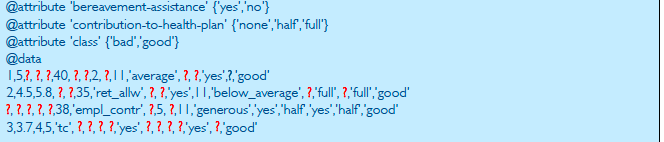
\includegraphics[width=.5\linewidth]{arffmissing}
%\end{figure}
Association rules are \textbf{frequent} patterns,associations,correlations or causal structures among sets of items or objects in databases. They are often used in basket data analysis,cross-marketing, catalog design and or any other application where matching similar or dissimilar items together based on an underlying relationship is important.\\Given a set of transactions the aim is to \textbf{find rules} that will \textbf{predict} the occurrence of an item based on the occurrence of \textbf{other} items in the transaction. Inside a \textbf{set of transaction} one can identify :
\begin{itemize}
\item \textbf{k-Itemsets}\\
An k-itemset is a collection of k items (e.g.$\{ bread,milk,jam\}, k=3$ )
\item \textbf{Support} \\
Fraction of transactions that contain an itemset (e.g. in a set of 8 transactions 3 contain itemset $\{ bread,milk,jam\}$ so support is $\frac{3}{8} $)
\item \textbf{Support count}\\
Frequency of occurrence of an itemset $\sigma(\{ Milk,Bread\})=3$
\item \textbf{Frequent itemset}\\
An itemset whose support is \textbf{greater than or equal to minsup threshold}.
\end{itemize} 
This way an \textbf{association rule} can be defined as an implication of the form $X \implies Y$ where X,Y are \textbf{itemsets}.
These rules can be evaluated by using 
\begin{itemize}
\item \textbf{Support s}\\
Fraction of transactions that contain both X (here Bread) and Y  (here Milk)
$$ s = \frac{\sigma(\{ Bread, Milk\})}{\text{num of transactions}}$$
\item \textbf{Confidence c}\\
Measures of often items Y appear in transactions that have X 
$$ c= \frac{\sigma(\{Bread,Milk\})}{\sigma(\{Bread\})}$$
\end{itemize}
The goal is to find , given a set of transactions T , associations rules having:
\begin{itemize}
\item Support $\geq$ minsup threshold
\item Confidence $\geq$ minconf threshold
\end{itemize}
To find associations rules \textbf{brute force} approach should \textbf{not} be used as it becomes easily computationally prohibitive.
\begin{figure}[H]
  \centering
  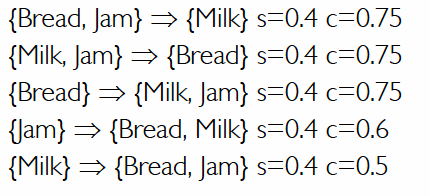
\includegraphics[width=.5\linewidth]{assrules}
\end{figure}
As seen in the figure above the rules all have same support as they are different partitions but with different confidence levels. This allows to \textbf{decouple} support and confidence:
\begin{enumerate}
\item Generate all itemsets whose support is $\geq$ minsup threshold (\textbf{Frequent itemset generation}).
\item Generate high confidence rules from frequent itemset where each rule is a binary partition of a frequent itemset ( \textbf{Rule generation}).
\end{enumerate}

\subsection{Frequent itemset generation}
Given d items there are $2^d$ possible \textbf{candidate datasets} which results in a huge complexity $\sim O(NMw)$
 \begin{figure}[H]
  \centering
  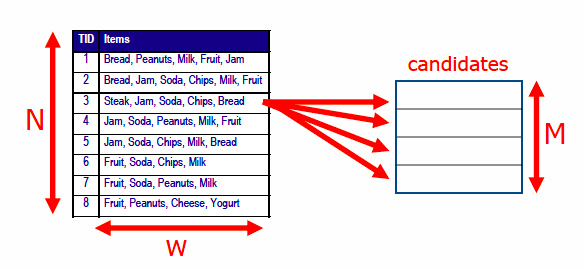
\includegraphics[width=.5\linewidth]{assbruteforce}
\end{figure}
To reduce the complexity : 
\begin{itemize}
\item Reduce number of candidates \textbf{M} by using \textbf{pruning} techniques
\item Reduce the number of transactions  \textbf{N} as size of itemset increases
\item Reduce number of comparisons \textbf{NM} by using efficient data structures and avoiding to match every candidate against every transaction.
\end{itemize}

\subsubsection{Apriori principle}
The Apriori principle states that if an itemset is \textbf{frequent} than all of its \textbf{subsets must also be frequent} (\textbf{anti-monotone property of support}) $$ \forall X,Y : (X \subseteq Y) \implies s(X) \geq s(Y)$$ 
 \begin{figure}[H]
  \centering
  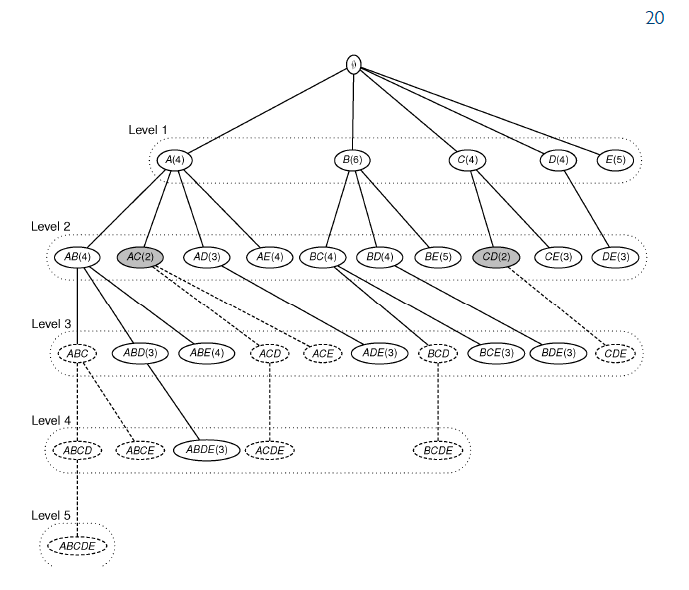
\includegraphics[width=.7\linewidth]{apriori}
\end{figure}
 \begin{figure}[H]
  \centering
  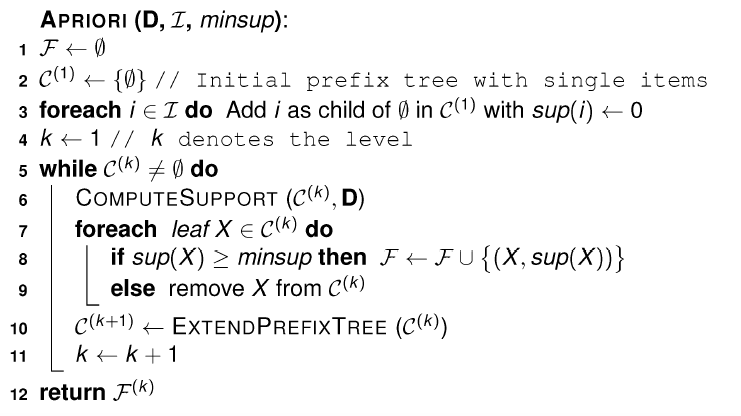
\includegraphics[width=.6\linewidth]{apriorialg}
\end{figure}

\subsubsection{Eclat}
Counting during support calculation creates a \textbf{bottleneck} which can be solved with this optimized algorithm. The algorithm works like the Apriori but for each itemset the \textbf{transaction ids} in which said itemset appears are saved too ( \textbf{tidset}). The following relationships applies :
$$ t(XY) = t(X) \land t(Y)$$
$$ sup(XY) = |t(XY)|$$
 \begin{figure}[H]
  \centering
  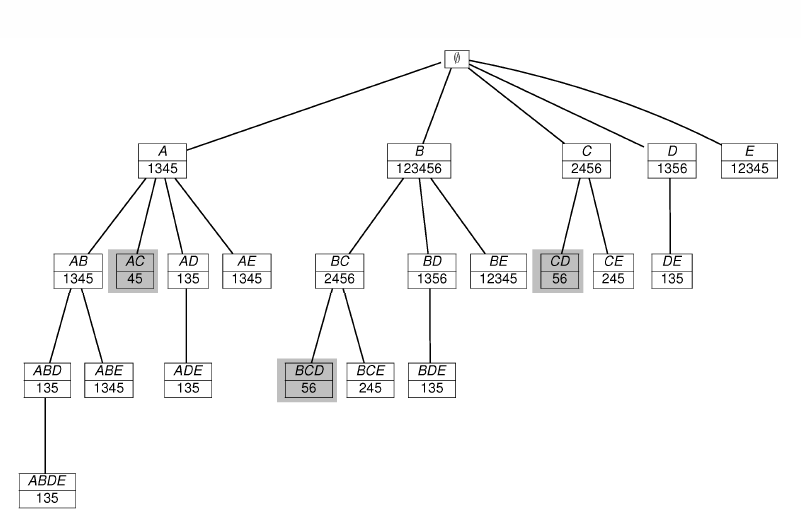
\includegraphics[width=.7\linewidth]{eclat}
\end{figure}

\subsubsection{Frequent pattern mining without candidate generation}
A big problem with frequent itemset mining is that they can be huge : a $10^4$ 1-itemset generates $10^7$ candidate 2-itemsets. To discover a frequent pattern of size 100 $\{a_1...a_100\}$ about $2^100 \sim 10^30$ candidates must be generated. The problem gets worse considering multiple database scan for support count.\\
The \textbf{Frequent Pattern Tree (FP Tree)} is a perfect solution to \textbf{compress} large databases \textbf{avoiding costly scans}. The generate-and-test phase from Apriori is completely dropped : 
\begin{enumerate}
\item Construct FP Tree
\item For each item i compute \textbf{projected FP tree}
\item Recursively mine conditional FP Trees and grow frequent patterns so far
\item If conditional FP tree has a \textbf{single path} then simply enumerate all the patterns
\end{enumerate}
 \begin{figure}[H]
  \centering
  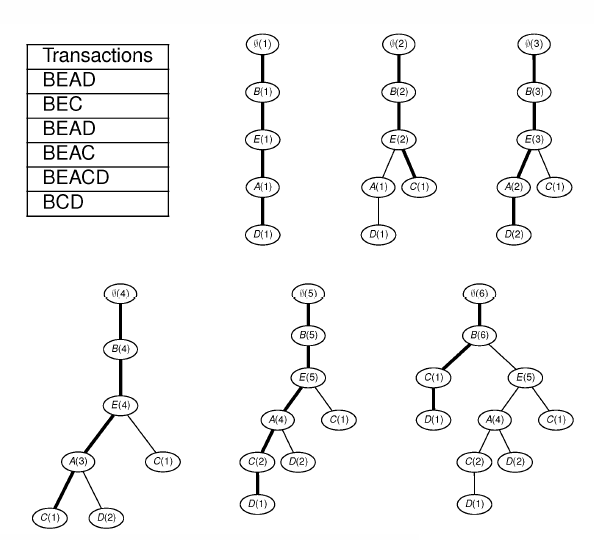
\includegraphics[width=.7\linewidth]{fptree}
\end{figure}
 \begin{figure}[H]
  \centering
  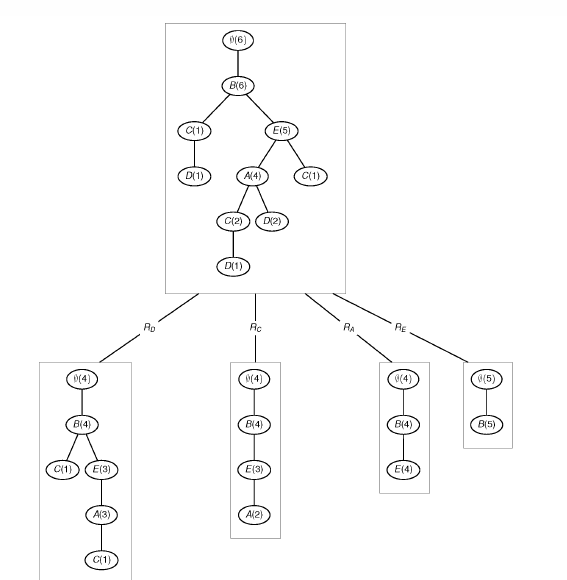
\includegraphics[width=.7\linewidth]{fptreecond}
\end{figure}
The method is:
\begin{itemize}
\item \textbf{Complete}\\
It preserves the information for frequent pattern mining and never breaks a long pattern of any transaction
\item \textbf{Compactness}\\
Reduces the relevant information (infrequent items are gone!) without ever exceeding the original database size. Items are in \textbf{frequency descending order}.
\end{itemize}

\subsection{Rule generation}
Given a frequent dataset L find all non-empty subsets $f \subset L$ such that $f \implies L-f$ satisfies \textbf{the minimum confidence requirement}. If $|L| = k \implies 2^K-2$ candidate association rules (ignoring $L \rightarrow \emptyset$ and $\emptyset \rightarrow L$).\\
Can rules be generated \textbf{efficiently} ? Confidence does not follow the \textbf{anti-monotone} property : 
$$ c(ABC \rightarrow D) \text{ can be larger than } c(AB \rightarrow D)$$
But is follows the anti-monotone property if rule are generated from the \textbf{same	 itemset}:
$$ L(\{ A,B,C,D\}) : c(ABC \implies D) \geq c(AB \implies CD) \geq c(A \implies BCD)$$
 \begin{figure}[H]
  \centering
  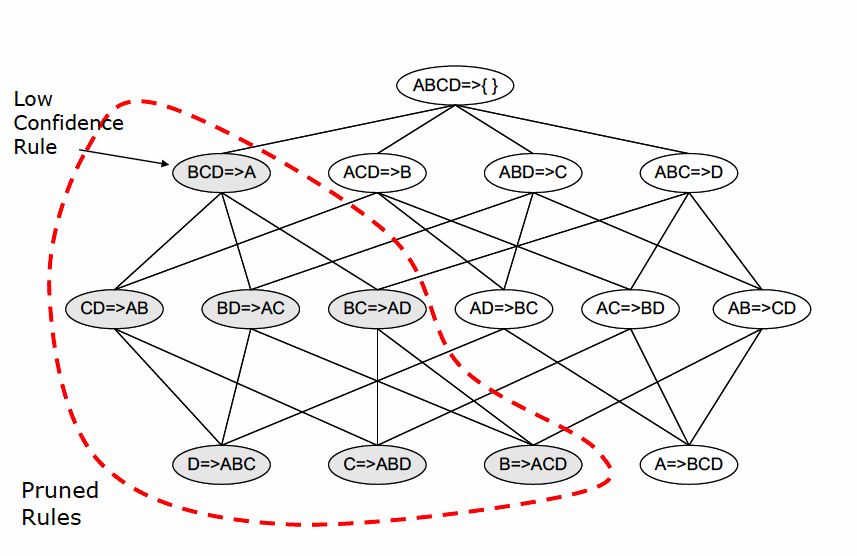
\includegraphics[width=.7\linewidth]{apriorirule}
\end{figure}
An example with min-conf = 9 :
 \begin{figure}[H]
  \centering
  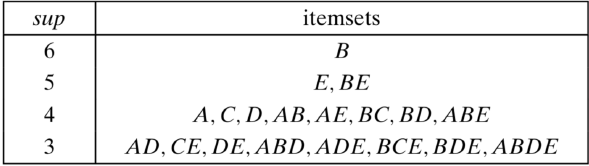
\includegraphics[width=.7\linewidth]{exrule}
\end{figure}
\begin{enumerate}
\item Start from largest itemset : \textbf{ABDE}
\item Generate all subsets \texttt{A}= $\{ ABDE, ABD,ABE...\}$
\item Starting from the first subset $X=ABD$ generate rule $ABDE \implies E$ with confidence $\frac{3}{3} > 0.9$.\\
Next one is $ABE \implies D$ with confidence $\frac{3}{4} < 0.9$.
\item Each time a subset has not met the required confidence level \textbf{all} of its \textbf{subsets} are \textbf{removed from} \texttt{A} (example remove all subsets of $ABE$ from \texttt{A}).
\item Finally the algorithm will output all the rules.
\end{enumerate}
 \begin{figure}[H]
  \centering
  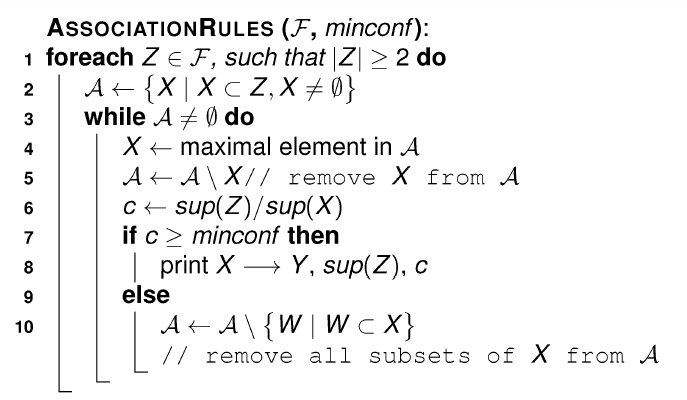
\includegraphics[width=.7\linewidth]{rulesalg}
\end{figure}

\subsection{Rule assessment measures}
If minsup is set \textbf{too high} itemsets involving interesting rare items could be missed ( like expensive products). On the other hand if it is set\textbf{ too low} the number of itemset gets very large : a \textbf{single} minimum threshold may not be sufficient ( applies for confidence too!).\\
\subsubsection{Lift}
Lift is the measure of the deviation of \textbf{stochastic independence} ( =1 then X and Y are independent) $$ \text{lift}(X \implies Y) = \frac{sup(X \cup Y)}{sup(X)sup(Y)}= \frac{conf(X \implies Y)}{sup(Y)}$$
It also measures the \textbf{surprise} of the rule : the closer to 1 means that the support of a rule is expected considering the support of its components. \\Useful lift values:
\begin{itemize}
\item $lift >> 1$ : rule \textbf{above} expectations
\item $lift << 1$ : rule \textbf{below} expectations
\end{itemize}

\subsubsection{Leverage}
Leverage gives an absolute measure of how surprising a rule is and should be used together with lift : $$\text{leverage}(X \implies Y )=sup(X \cup Y)-sup(X)sup(Y)$$

\subsection{Summarizing Itemsets}
When dealing with huge databases and itemset is there an efficient way to summarize them? There are some very technical measures :
\begin{itemize}
\item \textbf{Maximal frequent itemsets}\\
A \textbf{frequent} itemset is \textbf{maximal} has \textbf{no frequent supersets} :
$$ M = \{ X |X \in F \text{ and } !\exists Y \supset X \text{ such that } Y \in F \}$$
It gives a \textbf{condensed} representation as all subsets of the maximal itemset
 are \textbf{frequent}
\item \textbf{Closed Frequent itemsets}\\
An itemset X is \textbf{closed} if all supersets of X have \textbf{strictly less support} : 
$$ sup(X) > sup(Y) ,\text{ for all } Y \sup X$$
The set of \textbf{all} closed frequent itemsets is a \textbf{condensed} representation as we can determine whether an itemset X is frequent as well as the \textbf{exact} support of X  using C alone.
\item \textbf{Minimal generators}\\
A frequent itemset X is a minimal generator if it has \textbf{no subsets} with the same support $$ G = \{ X|X \in F \text{ and } !\exists Y \subset X , \text{ such that } sup(X) = sup(Y) \} $$ which means that $$ sup(X) < sup(Y)$$
\end{itemize}

\subsection{Mining frequent sequences}
Until now order was not considered. Sequences are often very important like in market basket analysis to know whether people buy items in sequence o discover navigation patterns on websites.\\
A \textbf{sequence} is an ordered list of symbols : $s = s_1,s_2,...s_k$ where $s_i$  or $s[i]$ denote the symbol at position i.
$$ \text{sequence: } s= s_1,...,s_n$$
$$ \text{sequence: } r=r_1,...,r_m$$
r is \textbf{subsequence} of s  ($r \subseteq s $) if there is a function $\phi$ from $[l,m]$ to $[l,n]$ such that $r[i] =s[\phi(i)]$ and for every position i,j in r : $i<j \implies \phi(i) < \phi(j)$ (order is maintained).\\
Subsequence r is \textbf{consecutive} if $r_1,r_2,...,r_m=s_j,s_{j+1},...,s_{j+m-1}$ \begin{figure}[H]
  \centering
  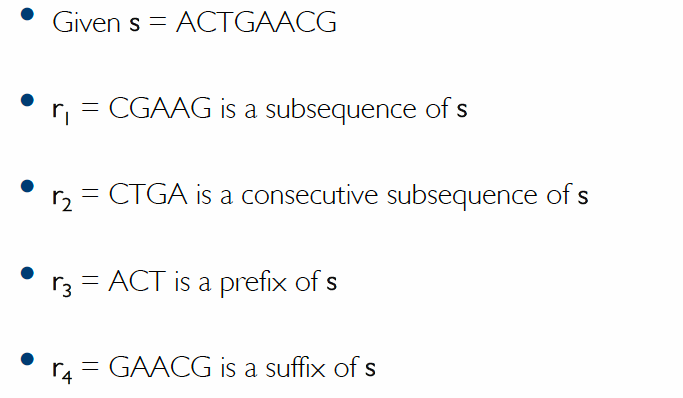
\includegraphics[width=.7\linewidth]{seqex}
\end{figure}
\begin{itemize}
\item \textbf{Sequence support}\\
Given a database \textbf{D} containing N sequences , the \textbf{support} of a sequence \textbf{r} in D is defined as the total number of sequences in D that contains r : 
$$ sup(r) = |\{ s_i \in D | r \subseteq s_i \}|$$
\item \textbf{Relative support}\\
The \textbf{relative support} is the percentage of sequences that contain r : 
$$ rsup(r) = \frac{sup(r)}{N}$$
\item \textbf{Frequent sequence}\\
A sequences is frequent if $sup(r) \geq minsup$
\end{itemize}

\subsubsection{Level-wise mining  GSP algorithm}
The GSP algorithm work in a similar fashion as the Apriori algorithm . It is a BFS algorithm.
\begin{enumerate}
\item Given a set of frequent itemsets at level k, the algorithm generates the candidate for level k+1 and computes the \textbf{support} of each candidate and prune the not frequent ones
\item For each sequence $s_i$ in D , check if a candidate \textbf{r} sequence is a \textbf{subsequence} of s (if yes  increment support of r). Then generate all k+1 level candidates
\item For each leaf $r_a$ the sequence is extended with the \textbf{last symbol} of any other leaf $r_b$ that shares the \textbf{same prefix} ( = same parent) so that $$ r_{ab} = r_a+r_b[k]$$ If $r_{ab}$ is infrequent then prune it.
\end{enumerate}

\subsection{Association rule for classification}
Given a dataset where classification can be performed ( for example data about patient with a class representing if a medicine has worked or not ). Association rules assume that the data have a transactional structure.Since classification tasks have data in tabular format , it is possible to find a mapping to perform classification with associations rules:
$$ X \implies c_i \quad c_i \text{ is a class label}$$
The confidence , for example , of $ X \implies class=yes $ represents the \textbf{conditional probability} $P(class=yes|...)$ so the confidence of the association rule is an evaluation of the predictive power (\textbf{CBA Algorithm}). It differs from normal association rules because we are working with \textbf{equalities} (like $outlook=sunny \implies ...$
\begin{figure}[H]
  \centering
  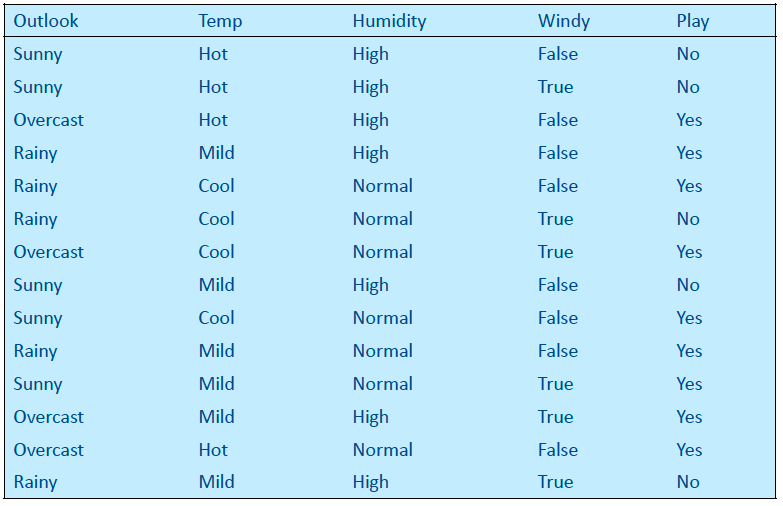
\includegraphics[width=.7\linewidth]{classrule}
\end{figure}
Here columns can take multiple values , for example $humidity = \{low,medium,high\}$ , which cannot be converted into a transactions that are used in association rule mining. A good solution is to use \textbf{One hot encoding}:
\begin{itemize}
\item $Humidity_low \in \{0,1\}$
\item $Humidity_medium \in \{0,1\}$
\item $Humidity_high \in \{0,1\}$

\end{itemize}